\documentclass[a4paper,10pt]{article}
\documentclass[a4paper,12pt]{report}
\usepackage[english]{babel}
\usepackage[left=2cm,right=2cm,top=2cm,bottom=2cm]{geometry}
%\usepackage{mathtools}
\usepackage{amsthm}     % for definitions and theorems
\usepackage[many]{tcolorbox}    % boxes around definitions and theorems
%\usepackage{amsmath}
%\usepackage{nccmath}
\usepackage{amssymb}    % \ltimes
\usepackage{etoolbox}   % for start of Chapter
%\usepackage{amsfonts}
\usepackage{physics}    % for all Physics related
\usepackage{dsfont}     % for the identity matrix symbol \1
%\usepackage{mathrsfs}

\usepackage{titling}
\usepackage{indentfirst}

\usepackage{bm}
\usepackage[dvipsnames]{xcolor}
\usepackage{cancel}

\usepackage{xurl}
\usepackage[colorlinks=true]{hyperref}

\usepackage{float}
\usepackage{graphicx}
\usepackage{subcaption}
%\usepackage{tikz}

\usepackage{ctable}     % tabelas
\renewcommand{\P}{\phantom{+}}  % empty space to indent things
\usepackage{multirow}
\usepackage{tabulary}

%%%%%%%%%%%%%%%%%%%%%%%%%%%%%%%%%%%%%%%%%%%%%%%%%%%

\newcommand{\eps}{\epsilon}
\newcommand{\vphi}{\varphi}
\newcommand{\cte}{\text{cte}}

\newcommand{\N}{{\mathbb{N}}}
\newcommand{\Z}{{\mathbb{Z}}}
%\newcommand{\Q}{{\mathbb{Q}}}
\newcommand{\C}{{\mathbb{C}}}
\renewcommand{\S}{{\hat{S}}}
%\renewcommand{\H}{\s{H}}

\renewcommand{\a}{{\vb{a}}}
\renewcommand{\b}{{\vb{b}}}
\renewcommand{\d}{{\dagger}}
\newcommand{\up}{{\uparrow}}
\newcommand{\down}{{\downarrow}}
\newcommand{\hc}{{\text{h.c.}}}

\newcommand{\ihat}{\bm{\hat{\imath}}}
\newcommand{\jhat}{\bm{\hat{\jmath}}}
\newcommand{\khat}{\bm{\hat{k}}}

\newcommand{\0}{{\vb{0}}}
\newcommand{\1}{\mathds{1}}
\newcommand{\E}{{\vb{E}}}
\newcommand{\B}{{\vb{B}}}
\renewcommand{\u}{{\vb{u}}}
\renewcommand{\v}{{\vb{v}}}
\renewcommand{\r}{{\vb{r}}}
\newcommand{\R}{{\vb{R}}}
\newcommand{\Q}{{\vb{Q}}}
\newcommand{\G}{{\vb{G}}}
\newcommand{\g}{{\vb{g}}}
\renewcommand{\k}{{\vb{k}}}
\newcommand{\K}{{\vb{K}}}
\newcommand{\p}{{\vb{p}}}
\newcommand{\q}{{\vb{q}}}
\newcommand{\F}{{\vb{F}}}
\renewcommand{\t}{{\vb{t}}}
\newcommand{\vtau}{{\bm{\tau}}}
\newcommand{\vdelta}{{\bm{\delta}}}

% COLORED SYMMETRY ELEMENTS
\newcommand{\Ct}{{\textcolor{Cyan}{C_3}}}
\newcommand{\Ctn}[1]{{\textcolor{Cyan}{C_3^{\textcolor{black}{#1}}}}}
\newcommand{\Cs}{{\textcolor{ForestGreen}{C_6}}}
\newcommand{\Csn}[1]{{\textcolor{ForestGreen}{C_6^{\textcolor{black}{#1}}}}}
\newcommand{\sd}{{\textcolor{RoyalBlue}{\sigma_d}}}
\newcommand{\sdn}[1]{{\textcolor{RoyalBlue}{\sigma_d^{\textcolor{black}{#1}}}}}
\newcommand{\sdp}{{\textcolor{RoyalBlue}{\sigma_d'}}}
\newcommand{\sdpp}{{\textcolor{RoyalBlue}{\sigma_d''}}}
\newcommand{\sv}{{\textcolor{Orange}{\sigma_v}}}
\newcommand{\svn}[1]{{\textcolor{Orange}{\sigma_v^{\textcolor{black}{#1}}}}}
\newcommand{\svp}{{\textcolor{Orange}{\sigma_v'}}}
\newcommand{\svpp}{{\textcolor{Orange}{\sigma_v''}}}

\newcommand{\s}{\sigma}
%\newcommand{\prodint}[2]{\left\langle #1 , #2 \right\rangle}
\newcommand{\cc}[1]{\overline{#1}}
\newcommand{\Eval}[3]{\eval{\left( #1 \right)}_{#2}^{#3}}
\newcommand{\sg}[2]{\{ #1 \mid #2 \}}

\newcommand{\unit}[1]{\; \mathrm{#1}}

\newcommand{\n}{\medskip}
\newcommand{\e}{\quad \mathrm{and} \quad}
\newcommand{\ou}{\quad \mathrm{or} \quad}
\newcommand{\virg}{\, , \;}
\newcommand{\ptodo}{\forall \,}
\renewcommand{\implies}{\; \Rightarrow \;}
%\newcommand{\eqname}[1]{\tag*{#1}} % Tag equation with name

\setlength{\droptitle}{-7em}

\makeatletter
\patchcmd{\chapter}{\if@openright\cleardoublepage\else\clearpage\fi}{}{}{}  % start 'Chapter' at the same page. needs package etoolbox
\makeatother

%% Theorems, definitions, proofs
\theoremstyle{definition}

\newtheorem{definition}{Definition}[section]
\tcolorboxenvironment{definition}{
  colback=blue!5!white,
  boxrule=0pt,
  boxsep=1pt,
  left=2pt,right=2pt,top=2pt,bottom=2pt,
  oversize=2pt,
  sharp corners,
  before skip=\topsep,
  after skip=\topsep,
}

\newtheorem{theorem}{Theorem}[section]
\tcolorboxenvironment{theorem}{
  colback=blue!5!white,
  boxrule=0pt,
  boxsep=1pt,
  left=2pt,right=2pt,top=2pt,bottom=2pt,
  oversize=2pt,
  sharp corners,
  before skip=\topsep,
  after skip=\topsep,
}


%\documentclass[../main.tex]{subfiles}
%\graphicspath{{\subfix{../fig/}}}

\begin{document}

\section{Commensurate Angles}


\begin{figure}[H]
\centering
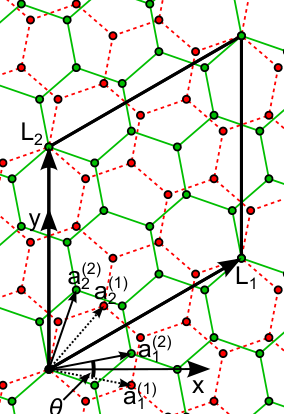
\includegraphics[width=0.4\textwidth]{fig/latvec.png}
\caption{Commensurate angle case and lattice vectors. Taken from \cite{koshino2012}}
\label{fig:latvec}
\end{figure}

As drawn in Figure \ref{fig:latvec}, we have
\begin{align}
\label{eq:scalarprods1}
\vb{a}_1^{(1)} \vdot \vb{a}_2^{(1)} &= a^2 \cos(60^\circ) = a^2/2; \\
\label{eq:scalarprods2}
\vb{a}_1^{(1)} \vdot \vb{a}_1^{(2)} &= a^2 \cos\theta; \\
\label{eq:scalarprods3}
\vb{a}_1^{(1)} \vdot \vb{a}_2^{(2)} &= a^2 \cos(60^\circ + \theta); \\
\label{eq:scalarprods4}
\vb{a}_1^{(2)} \vdot \vb{a}_2^{(1)} &= a^2 \cos(60^\circ - \theta).
\end{align}

The superlattice vectors $\vb{L}_1$, $\vb{L}_2$ (when the angle is commensurate) are related by a $60^\circ$ rotation. In general, because $\vb{L}_1$ is a point that belongs to the lattices of both layers, it is written by integers $m,n,m',n'$ as
\begin{equation} \label{eq:L1}
\vb{L}_1 = m\vb{a}_1^{(1)} + n\vb{a}_2^{(1)} = m'\vb{a}_1^{(2)} + n'\vb{a}_2^{(2)}.
\end{equation}

Koshino \cite{koshino2012} argues that there is an appropriate choice of lattice vectors $\vb{a}_1^{(1)}, \vb{a}_2^{(1)}, \vb{a}_1^{(2)}, \vb{a}_2^{(2)}$ (satisfying equations \ref{eq:scalarprods1} to \ref{eq:scalarprods4}) such that the indices $(m',n')$ can be made equal to $(n,m)$. If this is true, then by taking the scalar products of equation \ref{eq:L1} with $\vb{a}_1^{(1)}$ and $\vb{a}_1^{(2)}$, we get
$$
\begin{cases}
\; m + n/2 = n \cos\theta + m \cos(60^\circ + \theta); \\
\; m/2 + n = m \cos\theta + n \cos(60^\circ - \theta).
\end{cases}
\Rightarrow
\begin{cases}
\; mn + n^2/2 = n^2 \cos\theta + mn \qty(\frac{\cos\theta}{2}
- \frac{\sqrt{3} \sin\theta}{2}); \\
\; m^2/2 + mn = m^2 \cos\theta + mn \qty(\frac{\cos\theta}{2}
+ \frac{\sqrt{3} \sin\theta}{2}).
\end{cases}
$$

Summing the two equations above gives us
\begin{equation} \label{eq:costheta}
\boxed{\cos\theta = \frac{1}{2} \cdot \frac{m^2 + n^2 + 4mn}{m^2 + n^2 + mn}.}
\end{equation}


\pagebreak

\section{Moiré pattern}

By taking the norm of $\vb{L}_1$ from equation \ref{eq:L1} and using the angle relation in equation \ref{eq:costheta}, we find that the superlattice constant $L = \abs{\vb{L}_1} = \abs{\vb{L}_2}$ is given by
$$
2\sin[2](\theta/2) = 1 - \cos\theta = \frac{(m-n)^2}{2(m^2+n^2+mn)} \implies
\sqrt{m^2+n^2+mn} = \frac{\abs{m-n}}{2\sin(\theta/2)} \implies
$$
\begin{equation} \label{eq:}
L = a\sqrt{m^2 + n^2 + mn} = \frac{\abs{m-n}}{2 \sin(\theta/2)} \, a.
\end{equation}

\n


The area of an unit cell of the superlattice é $A = \frac{\sqrt{3}}{2} L^2 = (m^2 + n^2 + mn) \, A_1$, where $A_1 = \frac{\sqrt{3}}{2} \, a^2$ is the area of unit cell of monolayer graphene. If we consider now the area of the Brillouin Zone, we get
\begin{equation} \label{eq:bz-volume}
\Omega = \frac{\Omega_1}{m^2 + n^2 + mn},
\end{equation}
where $\Omega_1 = (2\pi)^2/A$ is the BZ area of the monolayer and $\Omega$ is the area of the moiré mini BZ.

\n

For example, $(m,n) = (1,2)$ and $\theta = 21.8^\circ$ we have $m^2 + n^2 + mn = 7$, therefore the monolayer BZ fits 7 mini BZ's in its area, as we see in Figure \ref{fig:bzminibz}.
\begin{figure}[H]
\centering
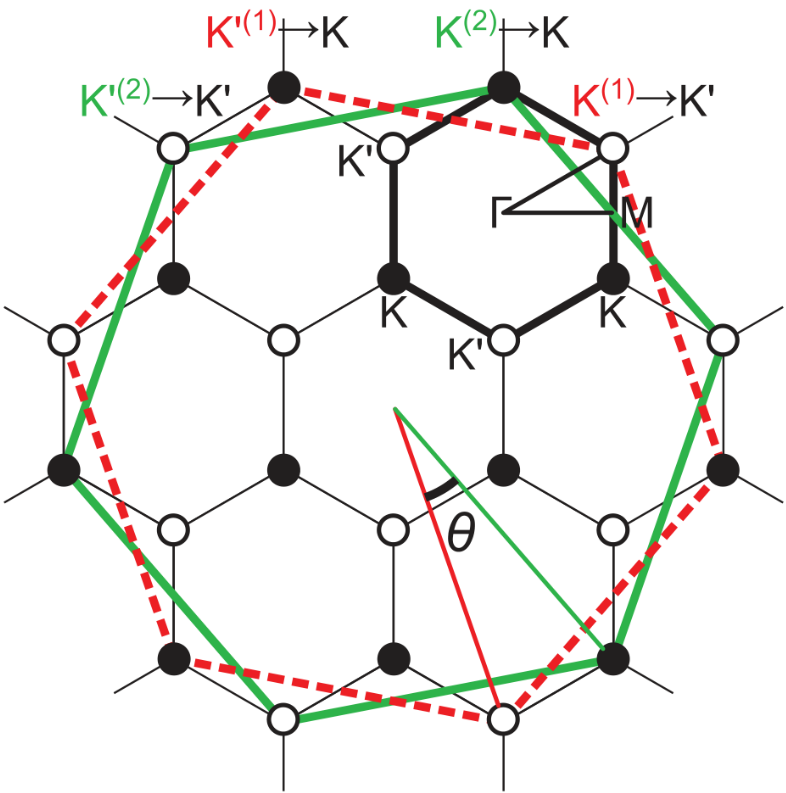
\includegraphics[width=0.5\linewidth]{fig/bzminibz.png}
\caption{Monolayers (red and green) and mini BZ's with $(m,n) = (1,2)$ and $\theta = 21.8^\circ$. Taken from \cite{koshino2012}.}
\label{fig:bzminibz}
\end{figure}

\n

\textbf{WHY DO WE ONLY CONSIDERER $\abs{m-n} = 1$?}

\pagebreak

\section{BM Model}

Here we will review the Bistritzer-MacDonald (BM) model \cite{macdonald2011}. First of all, the moiré pattern can be interpreted by a beat effect. Define the functions $h_\ell(\r)$, for each layer $\ell = 1, 2$, that describe their periodicity
$$
h_\ell(\r) = \sum_{k=1}^{3} \cos(\vb{G}_{\ell,k} \vdot \r),
$$
where the wave vectors $\vb{G}_{\ell,1} = \vb{b}_{\ell,1}$, $\vb{G}_{\ell,2} = \vb{b}_{\ell,2}$ and $\vb{G}_{\ell,3} = \vb{b}_{\ell,1} - \vb{b}_{\ell,2}$ give the directions for nearest neightbor hoppings in the hexagonal lattice. The moiré pattern will then be an interference between $h_1(\r)$ and $h_2(\r)$,
$$
h_{\text{moiré}}(\r) = h_1(\r) + h_2(\r) =
\sum_{k=1}^{3}
\, 2 \cos(\frac{\vb{G}_{1,k}+\vb{G}_{2,k}}{2} \vdot \r) \cos(\frac{\vb{G}_{1,k}-\vb{G}_{2,k}}{2} \vdot \r).
$$

The moiré pattern oscillates with $\vb{b}_k^{\text{moiré}} = \vb{G}_{1,k} - \vb{G}_{2,k}$, \cite{handbook2019}.

\n

Working on a coordinate system where the layer 2 is rotated by $\theta/2$ and layer 1 by $-\theta/2$, we have
$$
\vb{b}_1^{\text{moiré}} = \sqrt{3} \abs{\Delta K} \qty(\frac{1}{2}, -\frac{\sqrt{3}}{2}), \quad
\vb{b}_1^{\text{moiré}} = \sqrt{3} \abs{\Delta K} \qty(\frac{1}{2}, -\frac{\sqrt{3}}{2})
$$
<++>



%%-----
%% Referências bibliográficas
%%-----
\addcontentsline{toc}{chapter}{\bibname}
%\bibliographystyle{abntex2-num}
\bibliography{citations}
\bibliographystyle{ieeetr}


\end{document}
